\documentclass[8pt]{beamer}

\geometry{paperwidth=160mm,paperheight=120mm}

\usetheme[{titleformat plain}=smallcaps,
          titleformat title=smallcaps,
          titleformat subtitle=regular,
          titleformat section=smallcaps,
          titleformat frame=smallcaps,
          numbering=fraction
          ]{metropolis}
\usepackage{appendixnumberbeamer}

\usepackage{booktabs}
\usepackage[scale=2]{ccicons}

\usepackage{tikz}
\usetikzlibrary{shapes,arrows}
\usepackage{amsmath, bm}
\usepackage{siunitx}
\usepackage{physics,hepnames}
\usepackage{mathtools}
\usepackage{enumitem}

\usepackage{subfig}

\usepackage{pgfplots}
\usepgfplotslibrary{dateplot}

\usepackage{xspace}
\usepackage{soul}
\newcommand{\themename}{\textbf{\textsc{metropolis}}\xspace}

\DeclareMathOperator{\msbar}{\overline{MS}}
\DeclareMathOperator{\dis}{DIS}
\DeclareMathOperator{\phys}{PHYS}
\DeclareMathOperator{\pos}{POS}
\DeclareMathOperator{\dpos}{DPOS}
\DeclareMathOperator{\mpos}{MPOS}

\title{Can $\msbar$ PDF be negative?}
%\subtitle{arXiv:2006.07377}
\date{September, 2020}
\author{Alessandro Candido
}
%\institute{N3PDF}
\titlegraphic{
%        \raisebox{5pt}[0pt][0pt]{
\includegraphics[height=0.8cm]{../_logos/nnpdf_logo.pdf}}\hspace*{10pt}
        \hfill
        \raisebox{5pt}[0pt][0pt]{
\includegraphics[height=0.8cm]{../_logos/n3pdf_logo.pdf}}\hspace*{10pt}
        
\includegraphics[height=1.3cm]{../_logos/erc_logo1.png}

        \vfill\vspace*{190pt}
        
\includegraphics[height=1cm]{../_logos/unimi_logo.png}\hfill
        
\includegraphics[height=1cm]{../_logos/infn_logo.png}\\
        \vspace*{5pt}
        {\fontsize{3pt}{3.5pt}\selectfont
             \begin{center}
                 This project has received funding from the European Union's Horizon 2020 research and innovation programme under grant agreement No 740006\quad 
\includegraphics[height=5pt]{../_logos/eu-flag.jpg}
         \end{center}}
}

\begin{document}

\maketitle

\section{PDF @ NLO: factorization scheme}
\begin{frame}{NLO divergences}
    As well known at NLO divergences start to appear, both in virtual and real contributions.
    \begin{figure}
        \centering
        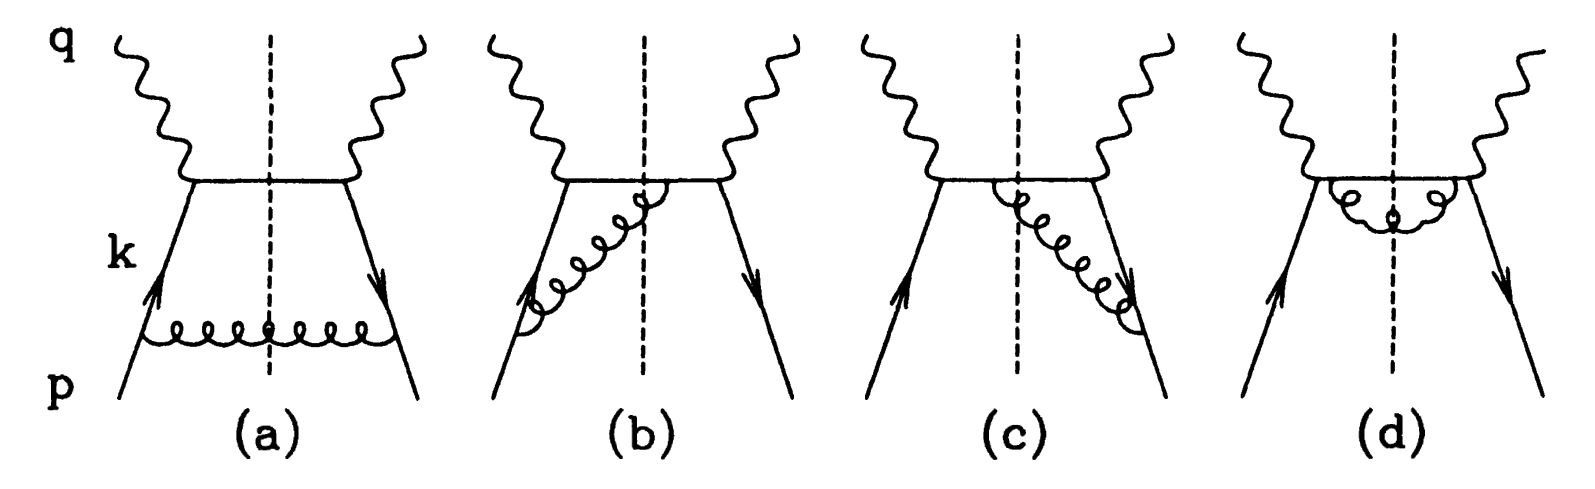
\includegraphics[width=.8\textwidth]{pictures/nlo-real}
    \end{figure}
    There are 3 kinds of divergences:
    \begin{itemize}
        \item \textbf{virtual}, due to loop integrals
        \item \textbf{soft}, due to emission of an extra soft particle
        \item \textbf{collinear}, due to the emission of an extra collinear particle
    \end{itemize}
    The first two kinds are known to cancel in sufficiently inclusive
    observables\footnote{e.g.: the KLN theorem is one of the results that guarantee
    this cancellation.}.
\end{frame}

\begin{frame}{NLO collinear divergences}
    On the other hand collinear divergences have \textit{a different origin}
    that can be related to the asymptotic freedom of strong interactions:

    \begin{center}
        \textit{The collinear limit corresponds to a long range (soft) part of
        the strong interaction, which is not calculable in perturbation
        theory.}
    \end{center}

    These divergences must be treated in a different way, defining a suitable
    \textbf{factorization scheme}.\newline

    Notice that collinear divergences are also responsible for the appearance
    of the characteristic $\alpha_s \log(Q^2)$, that will introduce the PDF
    dependency on $Q^2$.
\end{frame}

\begin{frame}{Factorization Scheme}
    \vspace*{15pt}
    The way to deal with these divergences is offered by the previous
    interpretation: we can hide them in a non-perturbative object, the PDF.
    \begin{align*}
        F_2(x,Q^2) &= x\sum_{q,\bar{q}} q_0 \otimes \hat{F}_{2,0} (x, Q^2) =
        x \sum_{q,\bar{q}} \int\limits_x^1 \frac{\dd\xi}{\xi} q_0(\xi)
        \hat{F}_{2,0}\left(\frac{x}{\xi},Q^2\right)\\
        &= x \sum_{q,\bar{q}} q \otimes \hat{F}_2 (x, Q^2)\\
    \end{align*}
    \vspace*{-15pt}

    Example: DIS scheme for DIS @ NLO
    \begin{align*}
        \hat{F}_{2,0}(x,Q^2) &= e_q^2 x \left[ \delta(1-x) +
        \frac{\alpha_s}{2\pi}\left(P(x) \log(\frac{Q^2}{\kappa^2}) +
        C(x)\right) + \dots \right]\\
        q(x, \mu^2_F) &= q_0(x) + \frac{\alpha_s}{2\pi} \int\limits_x^1
        \frac{\dd \xi}{\xi} q_0(\xi) \left\{ P\left(\frac{x}{\xi}\right)
        \log(\frac{\mu^2_F}{\kappa^2}) + C\left(\frac{x}{\xi}\right)\right\} +
        \dots
    \end{align*}
\end{frame}

\begin{frame}{Factorization Scheme}
    This will result:
    \begin{itemize}
        \item in the effective \textit{subtraction} of the collinear divergence
            in the partonic cross section
        \item the definition of a "renormalized" PDF
        \item the appearance of a new unphysical energy scale: $\mu_F$, the
            \textit{factorization scale} (which is on the same ground of $\mu_R$).
    \end{itemize}

    There is an \textbf{arbitrariness} on defining the finite part of the
    subtraction, in the very same way of the renormalization scheme.

    However, since the subtraction is related to a redefinition of the PDFs,
    once that a scheme has been \textbf{chosen} (fixing a finite subtraction)
    it should be kept for all the processes, because the \textbf{PDFs are
    always the same}.
\end{frame}

\begin{frame}{Factorization Scheme (CS counterterm)}
    The formula for a cross section in a generic factorization scheme can be
    written as an additional counterterm contribution $\dd\sigma^C_a$, in this
    case coming from the PDF redefinition:
    \begin{align*}
        \sigma_a^{NLO}(p; \mu_F^2) &= \int\limits_{m+1} \dd\sigma^R_a(p) +
        \int\limits_{m} \dd\sigma^V_a(p) + \int\limits_{m} \dd\sigma^C_a(p;
        \mu_F^2)\\
        \dd\sigma^C_a(p;\mu_F^2) &= - \frac{\alpha_s}{2\pi}
        \frac{1}{\Gamma(1-\epsilon)} \sum_b \int\limits_0^1 \dd z \left[ -
        \frac{1}{\epsilon} \left(\frac{4\pi\mu^2}{\mu_F^2}\right)^\epsilon
        P^{ab}(z) + K^{ab}(z) \right] \dd \sigma_b^B(zp)
    \end{align*}
    in dimensional regularization\footnote{The counterterm is such that
    $K^{ab}=0$ for $\msbar$ factorization scheme}.

    This will be useful in what follows, because it is exactly by choosing a
    specific factorization scheme (i.e. a specific $K^{ab}$ matrix) that we can
    analyze the property of the frequent $\msbar$ choice.
\end{frame}

\begin{frame}{Is there a positive scheme?}
    \begin{columns}
        \begin{column}{0.55\textwidth}
            At LO PDFs are positive by construction, but this is \textbf{not
            true at NLO}, since we \textbf{redefined the PDF} with the
            \textit{subtraction from the factorization scheme}.
            \newline

            Nevertheless it is easy to find a special class of
            \textbf{intrinsically positive} factorization schemes:
            the PDFs directly defined on \textbf{physical observables},
            subtracting \textit{all of the finite} contribution.
        \end{column}

        \begin{column}{0.45\textwidth}
            Like in the well-known DIS scheme we can choose two physical
            processes for defining the quark and gluon PDF:
            \begin{description}[style=unboxed]
                \item[quark] we can choose a hypothetical $\bar{q} p \to
                    \gamma^* + X$ (pure antiquark beam), or DIS;
                \item[gluon] either a hypothetical $g p \to H + X$ (pure gluon
                    beam), or a photon-gluon fusion;
            \end{description}
        \end{column}
    \end{columns}

    \vspace*{30pt}
    We can choose one of these schemes and call it $\phys$, for example:
    \begin{align*}
        \frac{1}{x}\bar{\sigma}(x,Q^2) &= f^{\,\phys}(x,Q^2)\\
        \bar{\sigma}(x,Q^2) &= \begin{pmatrix}
        \sigma(x,Q^2)[\bar{q} p \to \gamma^* + X]\\
        \sigma(x,Q^2)[g p \to H + X]
        \end{pmatrix}
    \end{align*}

    This scheme is positive by construction, since the PDF is proportional to a
    physical cross-section.
\end{frame}

\begin{frame}{Universality of collinear structure}
    \vspace*{15pt}
    \begin{columns}
        \begin{column}{0.45\textwidth}
            \begin{figure} \begin{tabular}{cc}
                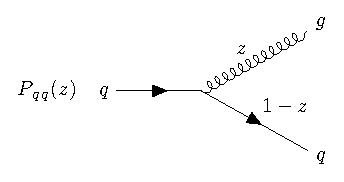
\includegraphics[width=0.45\textwidth]{pictures/feynd/Pqq} &
                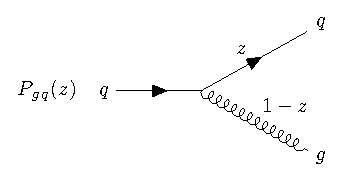
\includegraphics[width=0.45\textwidth]{pictures/feynd/Pgq} \\
                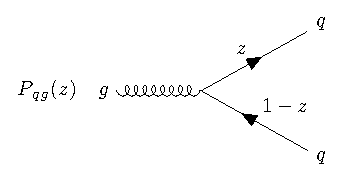
\includegraphics[width=0.45\textwidth]{pictures/feynd/Pqg} &
                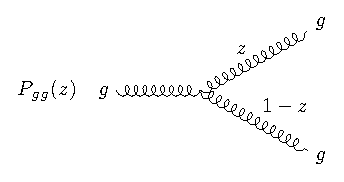
\includegraphics[width=0.45\textwidth]{pictures/feynd/Pgg} \\
            \end{tabular}
            %\caption{caption}
            \end{figure}

        \end{column}
        \begin{column}{0.55\textwidth}
            In $\msbar$ the subtracted cross section can be negative: negative
            finite parts are factored away from the regularized cross sections,
            into the PDFs, that can become negative as well.
            \newline

            On the other hand, the residue of the collinear pole is
            universal—it is given by process-independent splitting functions
            $P_{ab}$.
            \newline

            For this reason we can go on with the analysis of some particular
            process to catch the universal behavior involved in the
            factorization scheme.
        \end{column}
    \end{columns}

    \vspace*{15pt}
    \textbf{\large The problem}

    \begin{columns}
        \begin{column}{0.4\textwidth}
            The original $d$-dimensional expression is positive by construction, since
            it is a \textbf{cross-section}, but the $\msbar$ prescription leads to an
            over-subtraction in the gluon channel.

        \end{column}
        \begin{column}{0.6\textwidth}
            \begin{figure}
              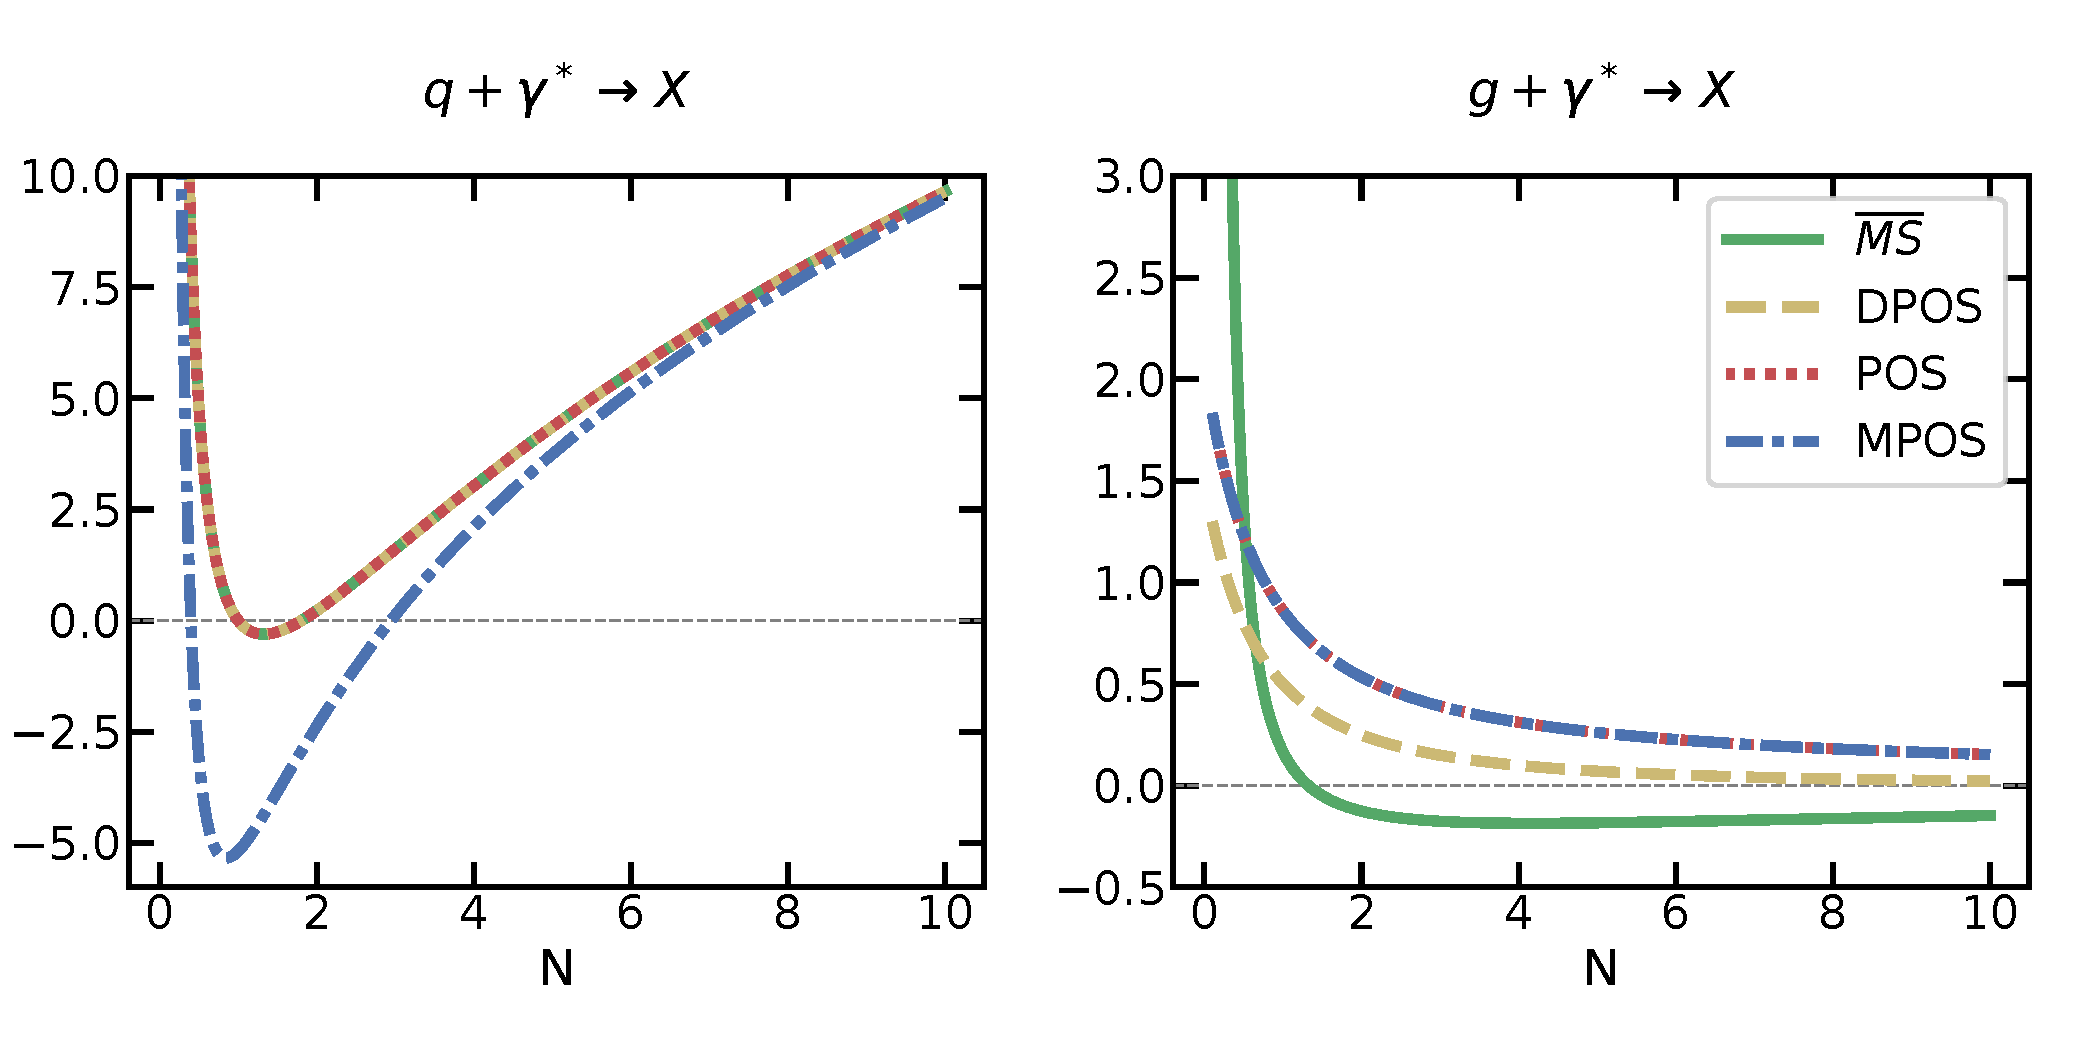
\includegraphics[width=0.95\textwidth]{pictures/dis}
            \end{figure}
        \end{column}
    \end{columns}
\end{frame}

\begin{frame}{DIS coefficient functions}
    \begin{block}{Gluon channel}
    \vspace*{1pt}
    We can make it positive again analyzing the source of over-subtraction.
    \end{block}

    \begin{align*}
        {C^{(1)}_{g}}^{\msbar}(x) &= \lim_{\epsilon\to
        0^-}\left[C_{g}^{(1)}(x,Q^2,\epsilon) - \left(\frac{Q^2}{4\pi
        \mu^2}\right)^{-\epsilon} \left(-\frac 1
        {\epsilon}+\gamma_E\right) P_{qg}(x)\right]\\
        {C^{(1)}_{g}}^{\dpos}(x) &= \lim_{\epsilon\to0^-}
        \left[{C^{(1)}_{g}}(x,Q^2,\epsilon) -
        \frac{1}{\alert{1-\epsilon}}\left(\frac{\alert{\mu_D^2}}{\pi\mu^2}\right)^{-\epsilon}
        \left(-\frac 1 {\epsilon}+\gamma_E\right) P_{qg}(x)\right]\\
        \mu_D^2&\equiv|k_T^{\text{max,\,DIS}}|^2=\frac{s}{4}=\frac{Q^2(1-x)}{4x},
    \end{align*}

    The changes applied have an intrinsic physical meaning:
    \begin{itemize}
        \item the $\dpos$ scheme is subtracting at correct energy scale
            (maximal transverse momentum, not virtuality)
        \item d-dimensional gluon polarizations' average is taken into
            account
    \end{itemize}

    \vspace*{5pt}
    From the definitions of $\msbar$ and $\dpos$ it is possible to define a
    \textit{change of scheme} matrix $K$:
    \begin{equation*}
      K_{qg}^{\dpos}(x)= {C^{(1)}_{g}}^{\msbar}(x) - {C^{(1)}_{g}}^{\dpos}(x) = P_{qg}(x)\left[\log(\frac{1-x}{x}) - 1\right]
    \end{equation*}

    \begin{block}{Quark channel}
    \vspace*{1pt}
    Since in this case it would be an \textit{under-subtraction} for the sake
    of positivity it is fine to choose $K_{qq}^{\dpos}(x) = 0$.
    \end{block}
\end{frame}


\begin{frame}{Incoming gluon and Hadronic processes}
    \begin{columns}
        \begin{column}{0.5\textwidth}
            Still to do:
            \begin{itemize}
                \item there are still two elements of matrix missing
                    $K_{qg}^{\dpos}(x)$ and $K_{gg}^{\dpos}(x)$, so we need a
                    process with an incoming gluon at LO.

                \item the factorization scheme is linked to collinear
                    structure, that is universal \textit{w.r.t. the hard
                    process}, but is affected by the \textbf{incoming
                kinematics}.
            \end{itemize}

            \vspace*{8pt}
            A suitable process for both is $gg\to h + X$ in HEFT:
            \begin{figure}
              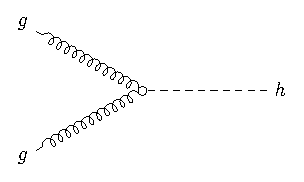
\includegraphics[width=0.55\textwidth]{pictures/feynd/ggh}
            \end{figure}
        \end{column}
        \begin{column}{0.5\textwidth}
            The only difference is just in the incoming kinematics\footnotemark.
            This yields that the only new thing is just the \textbf{different energy available
            for transverse momentum}:
            \begin{equation*}\label{eq:ktmaxh}
                \mu_h^2=  |k_T^\text{max, had}|^2=\frac{(s-Q^2)^2}{4s}=\frac{Q^2(1-x)^2}{4x}
            \end{equation*}
            where $x=\frac{M_H^2}{s}$ and $ Q^2 = M_H^2 $.

            \vspace*{10pt}
            The \textbf{off-diagonal} matrix element it is similar to the DIS, but
            with a further contribution coming from the second incoming particle
            \begin{equation*}
                K_{gq}^{\pos} (x) =
                P_{gq}(x)\left[\ln\left(\frac{(1-x)^2}{x}\right) - 1\right]
            \end{equation*}
            and $K_{gg}^{\pos} (x) = 0$
        \end{column}
    \end{columns}
    \footnotetext{Process specific ingredients are not involved in PDFs
    factorization.}

    \vspace*{15pt}
    \textbf{\large $\pos$ for both}
    
    We changed to $\pos$ applying the same energy correction $\mu_h^2$ in all
    the channels (instead of $\mu_D^2$).

    Since the $\pos$ scheme results to make the DIS cross-sections even more
    positive (non minimal subtraction) it is a good candidate for a positivity
    scheme.
\end{frame}


\begin{frame}{Is $\msbar$ negative? (non-singlet)}
    First of all we can consider the case of a \textbf{non-singlet} PDF:
    $q^{\text{NS}}(x, Q^2) = q_i(x, Q^2) - q_j(x, Q^2)$
    \footnote{This is \textit{academic} because we are going to \textbf{assume
    it positive in a physical scheme}, but being a \textit{difference} it may
    also not exist such a positive non-singlet.}.

    \vspace*{10pt}
    Master formula for this part of the argument is:
    \begin{equation*}
        \left[{q^{\text{NS}}}\right]^{\text{DIS}}(x,Q^2)=
        \left[1+\frac{\alpha_s}{2\pi} {\Delta^{(1)}_q}^{\msbar}
        +\frac{\alpha_s}{2\pi}  {\bar
        C^{(1)}_q(x)}^{\msbar}\otimes\right]\left[{q^{\text{NS}}}\right]^{\msbar}(Q^2)
    \end{equation*}

    \vspace*{20pt}
    \textbf{\large Positivity with a single PDF $\iff C_q(x)^{\msbar} > 0$}
    \vspace*{14pt}

    \begin{columns}
        \begin{column}{0.5\textwidth}
            \textbf{Necessity}
            \newline

            Since DIS PDFs are known to be positive, being physical, but
            assuming a generic positive $\msbar$ PDF without any other
            restriction yields the coefficient function to be
            positive\footnotemark.
        \end{column}
        \begin{column}{0.5\textwidth}
            \textbf{Sufficiency}
            \newline

            Applying a \textbf{perturbative inversion} to the master formula,
            since physical (here $\text{DIS}$) PDF is
            positive and perturbatively the coefficient
            cannot become negative\footnotemark.\\
        \end{column}
    \end{columns}
    \footnotetext[6]{Like in a variational argument one assumes the
    coefficient of the variation to be zero, since the variation can be
    whatever.}
    \footnotetext{There is a single \textit{caveat}: in the region $x \to 1$ it's not perturbative,
    so in this case the inverted formula to $\text{LL}(1-x)$.}
\end{frame}

\begin{frame}{Is $\msbar$ negative? (singlet-gluon system)}
    Instead singlet and gluon are coupled
    \begin{equation*}
        \frac{1}{x} \sigma(x,Q^2)= \hat \Sigma_0\otimes \left[1
        +\frac{\alpha_s}{2\pi}  C^{(1)} \otimes \right] f(Q^2) \,.
    \end{equation*}
    where:
    \begin{equation*}
        \sigma(x,Q^2)=\left(\begin{array}{c} \sigma^{q}(x,Q^2)\\ \sigma^{g} (x,Q^2)\end{array}\right) \qquad
        \hat \Sigma_0(x,Q^2)=\left(\begin{array}{cc} \hat \sigma_0^{q} q (x,Q^2) &
                  0 \\0 & \sigma_0^{g} g (x,Q^2) \end{array}\right) \qquad
          f(x,Q^2)=\left(\begin{array}{c} q(x,Q^2) \\ g(x,Q^2) \end{array}\right)
    \end{equation*}
    so $\sigma$ represents a couple of processes, and the coefficient function
    is a two-by-two matrix.

    The only new ingredients are \textbf{off-diagonal terms}, but $\pos$ has
    been defined taking explicitly care of them.
    So the argument it's pretty the same, but to apply it one should consider a
    pair of processes.

    \vspace*{15pt}
    \textbf{\large To a positive $\msbar$}

    With $\pos > 0$ he prove of $\msbar > 0$ is straightforward, since the
    explicit transformation between the two schemes is known:
    \begin{equation*}
        \hspace*{-12pt}\left[\mathbb{I}
        +\frac{\alpha_s}{2\pi} {C^{(1)}}^{\msbar}\right]=\left[\mathbb{I}
          +\frac{\alpha_s}{2\pi} {C^{(1)}}^{\pos}
          \right]\left[\mathbb{I}
          + \otimes \frac{\alpha_s}{2\pi}  K^{\pos}\right]
    \end{equation*}
    and so:
    \begin{equation*}
     f^{\,\pos}(Q^2)=\left[\mathbb{I}
      +\frac{\alpha_s}{2\pi}  K^{\pos}\otimes\right] f^{\,\msbar}(Q^2)\,,
    \end{equation*}
    which \textbf{inverse} can be obtained \textbf{perturbatively} (with the
    same caveat for the $x \to 1$ \textbf{limit}).
\end{frame}

\begin{frame}{Conclusions}
    \begin{columns}
        \begin{column}{0.6\textwidth}
        \textbf{\large Is it enough?}
        \vspace*{10pt}

        No it's \textbf{not enough}, \textbf{nor needed}.
        \metroset{block=fill}
        \begin{block}{Sufficient}
         PDF positivity it's still not enough to guarantee observables
         positivity, since the coefficient functions are not bounded to be
         positive in x space in 4 dimensions.
        \end{block}

        \begin{block}{Necessary}
        It's also not necessary, because negative PDF folded with suitable
        coefficient functions can still lead to positive observables.
        \end{block}

        \end{column}

        \begin{column}{0.4\textwidth}
        \textbf{\large So why?}

        \vspace*{10pt}
        It is a useful physical constraint on the PDFs, so it will add
        \textbf{more theoretical knowledge} in the fit.

        In practice it cuts out a region of the hypothesis space that should not be
        explore by the fitting algorithm, so


        \end{column}
    \end{columns}

    \vspace{20pt}
    \begin{center}
        \textit{The main result will be reducing the variance of the fitted PDFs.}
    \end{center}

    %\vspace*{25pt}
    %\metroset{block=fill}
    %\begin{block}{Further scheme optimization}
        %It is natural to ask whether the positivity requirement could be more
        %restrictive in some factorization schemes than others, but it is
        %unclear  whether  and  how  this  question  could  be  answered.
    %\end{block}

\end{frame}

\begin{frame}[standout]
    Thanks for your attention
\end{frame}

\appendix

%\begin{frame}{Overall structure of the argument}
    %\begin{enumerate}
        %\item $\msbar$ partonic cross-sections are not positive, we found why
            %not a define a factorization scheme that prevent it
        %\item enforce momentum sum rules by slightly modifying the former,
            %without affecting positivity
        %\item considering the scheme change we prove that positivity of PDFs in
            %this last scheme prove positivity of PDFs in $\msbar$
    %\end{enumerate}
%\end{frame}

%\begin{frame}{Positive coefficient functions}
    %A subtlety is related to the fact that generally partonic cross sections
    %are the sum of an ordinary functionof the scaling variable, and a
    %distribution localized at the kinematic threshold of the scaling variable.
    %Here,by “negative cross section” we mean that the function (i.e.,
    %non-distributional part of the cross section) isnegative.  For positivity
    %to hold,  the distributional part must also be positive in the sense that
    %it gives apositive result when integrated over a positive test function.
    %As we shall see below, this condition turns outto be automatically
    %satisfied inMS and related schemes
%\end{frame}

%\begin{frame}{$\pos$ scheme}
%POS scheme:
%\begin{align*}
 %{{C^q{}_q}^{(1)}}^{\pos}(x) &=  {{C^q{}_q}^{(1)}}^{\msbar}(x) \,, \\
 %{{C^q{}_g}^{(1)}}^{\pos} (x) &=  {{C^q{}_g}^{(1)}}^{\msbar} (x) - K_{qg}^{\pos} (x) \,,\\
  %K_{qg}^{\pos} (x) &=  P_{qg}(x)\left[\log(\frac{(1-x)^2}{x}) - 1\right] \,.
 %{{C^g{}_g}^{(1)}}^{\pos}(x)  &=  {{C^g{}_g}^{(1)}}^{\msbar}(x) \,, \\
 %{{C^g{}_q}^{(1)}}^{\pos} (x) &=  {{C^q{}_g}^{(1)}}^{\msbar} (x) - K_{gq}^{\pos} (x) \,,\\
  %K_{gq}^{\pos} (x) &=  P_{gq}(x)\left[\log(\frac{(1-x)^2}{x})- 1\right]
%\end{align*}
%Hence, subtraction in the
%DPOS scheme amounts to under-subtraction, and if adopted for DIS
%coefficient function it leads to a DIS coefficient function
%${C^{(1)}_{g}}^{\pos}(x)$ which is actually more positive than that
%in the DPOS scheme. This is seen in Fig.~ (right), where
%${C^{(1)}_{g}}(x)$ is shown in the $\msbar$, DPOS and POS schemes.
%\end{frame}

%\begin{frame}{N-space positivity $\neq$ x-space positivity}
    %The easy way in \textit{N-space} and Why we need an argument in \textit{x-space}
%\end{frame}

%\begin{frame}{Non-singlet}
    %\begin{description}
        %\item[academic] it can be that no positive non-singlet combination
            %exists, since it is the subtraction of quarks distributions for two
            %different flavors;
        %\item[isolated] the same we used the non-singlet to set up the argument
            %since the singlet is slightly more complicated, indeed the gluon
            %couples to all the flavors in the same way, so any correction
            %coming from the gluon-quark mixing in change of scheme is
            %annihilated by the non-singlet combination;
    %\end{description}
%\end{frame}

%\begin{frame}{NLL calculation}
    %The calculation in $x \to 1$ limit, better not to include in the main body (eq. 50-53)
%\end{frame}

%\begin{frame}{To a positive $\msbar$}
    %The explicit expression of the change of scheme matrix $K$ is:
    %\begin{equation*}
        %K^{\pos}=\left[\ln\left(\frac{(1-x)^2}{x}\right) - 1\right]
        %\left(\begin{array}{cc} 0 & P_{qg}(x) \\
        %P_{gq}(x) & 0\end{array}\right).
    %\end{equation*}
    %and its shape in $N$-space can be plotted:
    %\begin{figure}
      %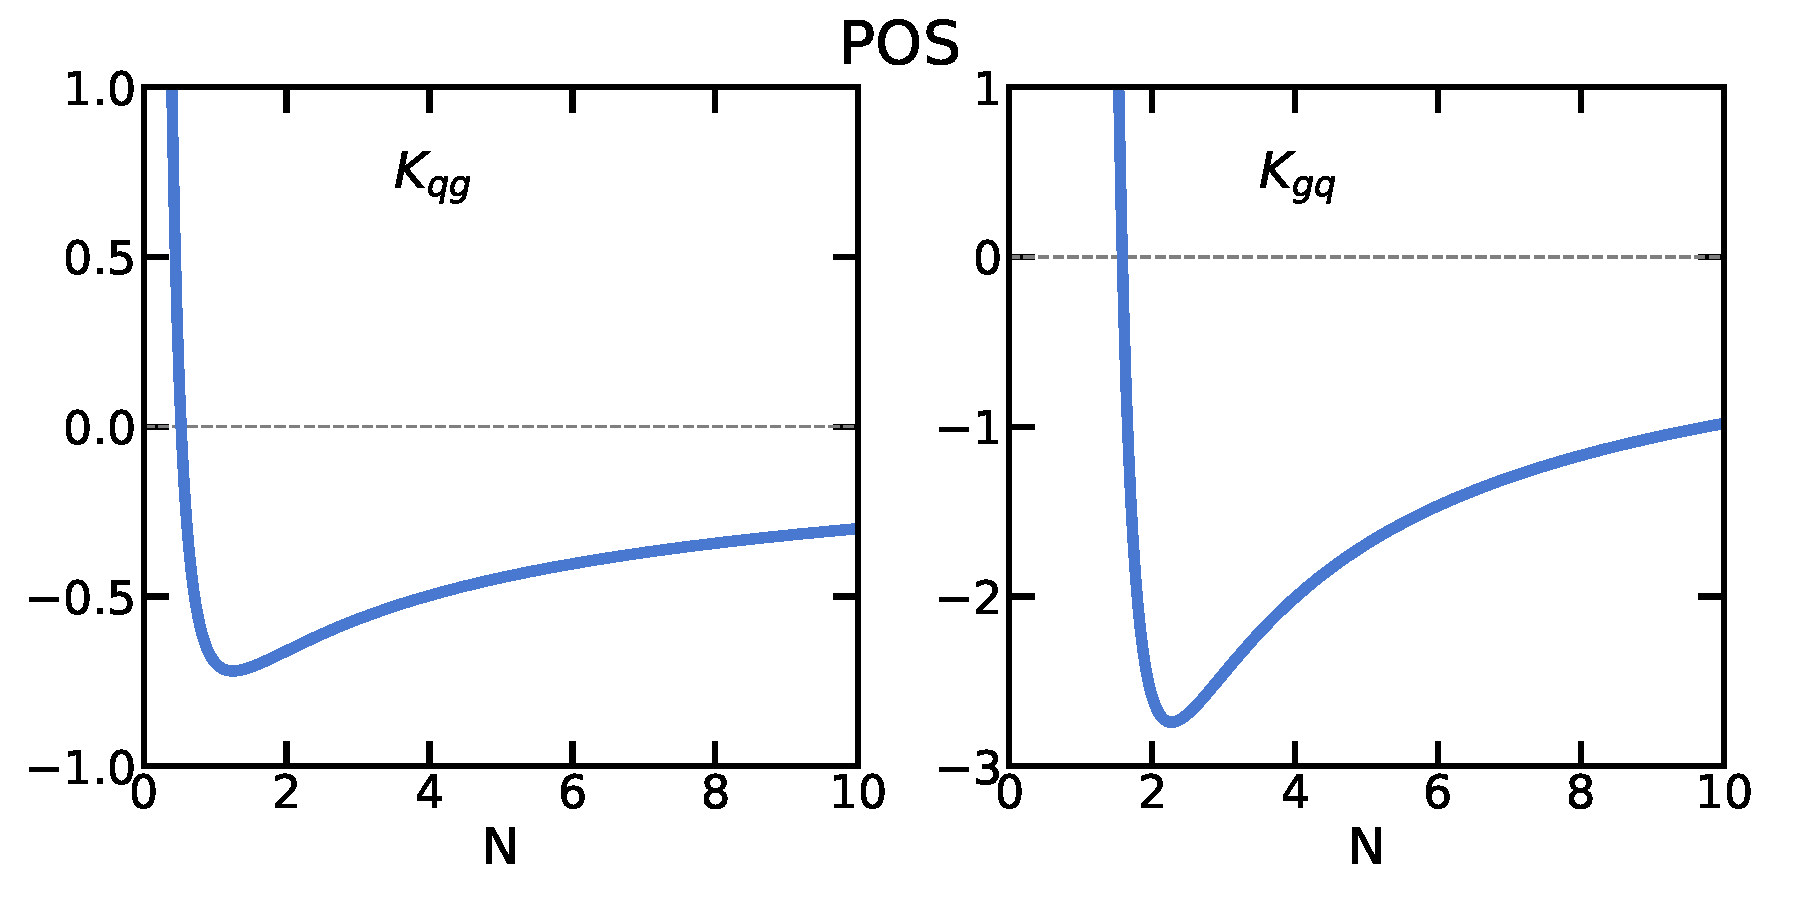
\includegraphics[width=0.75\textwidth]{pictures/kmatrix-offdiagonal-9}
    %\end{figure}
%\end{frame}

%\begin{frame}{Momentum Sum Rules}
    %Inspection of Eq. immediately shows a possible issue
    %with the POS scheme. Indeed, as well known, momentum conservation
    %implies the pair of relations between the second Mellin moments of splitting
    %functions $\gamma_{qq}(2)+\gamma_{gq}(2)=0$ and
     %$2n_f\gamma_{qg}(2)+\gamma_{gg}(2)=0$. This relation is verified in the
    %$\msbar$ scheme:  in order for it to remain true  in any scheme obtained
    %from $\msbar$, the scheme change matrix must satisfy
    %\begin{equation}\label{eq:momcons}
      %K_{qq}+K_{gq}=2n_fK_{qg}+K_{gg}\Big|_{N=2}=0 \,,
    %\end{equation}
    %where by $K_{ij}\Big|_{N=2}$ we denote the second Mellin moment of the
    %scheme change matrix elements. This relation is not satisfied by the matrix defined in
    %Eqs.

    %It might therefore be worth considering a variant of the POS scheme,
    %in which momentum conservation is enforced by adding to the diagonal
    %elements of the scheme change matrix a contribution which enforces
    %momentum conservation. This can be done e.g.\ by adding a soft
    %function, which vanishes both as $x\to1$ and $x \to0$. We choose
    %\begin{equation}\label{eq:fmom}
      %f^{\text{MOM}}(x)= 60 x^2(1-x)^2\,,
    %\end{equation}
    %which has the property that its second Mellin moment equals one:
    %$f^{\text{MOM}}(N=2)=1$. We then define a MPOS scheme as that which is obtained
    %from $\msbar$ through a scheme change matrix $K^{\mpos}$ whose
    %matrix elements satisfy
    %\begin{align}
      %\label{eq:mposqq}
      %K^{\mpos}_{qq}(x)&= - f^{\text{MOM}}(x) K^{pos}_{gq}\Big|_{N=2} \,,\\
      %\label{eq:mposqg}
      %K^{\mpos}_{qg}(x)&= K^{pos}_{qg}(x) \,,\\
      %\label{eq:mposgq}
      %K^{\mpos}_{gq}(x)&= K^{pos}_{gq}(x) \,,\\
      %\label{eq:mposgg}
      %K^{\mpos}_{gg}(x)&= -2n_f f^{\text{MOM}}(x) K^{pos}_{qg}\Big|_{N=2} \,.
    %\end{align}
    %The MPOS scheme then automatically satisfies momentum
    %conservation. Coefficient functions in the MPOS scheme are shown in
    %Figs.~. It is clear that coefficient
    %functions, and thus PDFs, remain
    %positive in the MPOS scheme: indeed, the off-diagonal coefficient
    %functions are unchanged, while the diagonal NLO contributions are
    %modified by a small correction which is offset by the large positive
    %LO contribution, and in fact in the hadronic case leaves the NLO
    %correction positive for all $x$. Hence the MPOS and POS schemes have the same
    %positivity properties. We will thus not discuss the MPOS scheme
    %any further and restrict the discussion for simplicity to the POS
    %scheme.
%\end{frame}

%\begin{frame}{Heavy quarks}
    %Heavy quarks require a separate discussion,  because their factorization
    %scheme can bedefined in a variety of ways (see e.g. [19]).  Specifically,
    %heavy quarks can be treated in amassive scheme,  in which collinear
    %singularities associated to them are regulated by theirmass, so they decouple
    %from perturbative evolution. In this scheme no collinear subtraction
    %isperformed for massive quarks, so their PDF is given by the unsubtracted Eq.
    %(2) and thus itremains a positive (and scale-independent) probability
    %distribution to all perturbative orders.Note that nothing prevents this heavy
    %quark PDF from having an “intrinsic” component, ofnon-perturbative origin:
    %however, in this factorization scheme, the heavy quark PDFs willbe
    %scale-independent, and thus positive at all scales.

    %However, it is also possible to treat the heavy quark in a massless scheme,
    %in which theheavy quark is treated like other massless quarks, namely the
    %collinear singularity regulatedby its mass is subtracted according to Eqs.
    %(9,20), but withμ2now replaced by the heavyquark mass.  Calculations performed
    %in this scheme, with heavy quark mass effects neglected,are accurate for scales
    %much larger than the quark mass.  ForQ2m2hthis scheme reducesto the standardMS
    %and the previous arguments apply.  However, the massless scheme is inprinciple
    %formally defined for all scales, including at the heavy quark mass. This is
    %sometimesdone by using the massless scheme for all flavors, but discontinuously
    %changing the number offlavors at a matching scale chosen equal to (or of order
    %of) the heavy quark mass (zero-massvariable-flavor number scheme,  ZM-VFNS
    %[20]).  Below the matching scale the ZM-VFNSscheme  coincides  with  the
    %massive  scheme  (with non-evolving  heavy  quark  PDF),  and  atthe matching
    %scale the heavy quark PDF changes discontinuously:  the matching condition20 is
    %the scheme transformation from the massive to the masslessMS (computed up to
    %NNLOin  Ref.  [21]).   At  this  scale,  the  scheme  change  matrix  from  the
    %(positive) massive  flavorto massless scheme is a function of the heavy quark
    %massmh, rapidly varying with scaleqwhenQ∼mhand unrelated to the scheme change
    %fromMS to POS. Hence, the previousarguments do not apply and no conclusions can
    %be drawn on on the positivity of the heavy-quark PDF in the massless scheme
    %from its positivity in the massive scheme.  Indeed,  forrealistic quark and
    %gluons and in the absence of intrinsic component theMS massless-schemecharm PDF
    %turns out to be negative for somexvalues when the scale is set equal to
    %thecharm mass
%\end{frame}

%\begin{frame}{Positive to all orders}
    %All the discussion so far has been pursued at NLO.  However, the main
    %structure of theargument remains true to all perturbative orders.  In
    %particular, it is true to all orders thatthe diagonal splitting functions
    %are negative at largex:  in fact, at largexto all perturbativeorders they
    %behave as1(1−x)+[14].  At higher perturbative orders, coefficient functions
    %willcontain higher order powers of ln(1−x), leading to the familiar rise in
    %the partonic crosssection  which  is  predicted  to  all  orders  by
    %threshold  resummation  [11, 12].   Off-diagonalchannels,  where  negative
    %contributions  asx→1  may  and  indeed  are  expected  to  arise,remain
    %power  suppressed  in  this  limit.   It  follows  that  the  off-diagonal
    %structure  Eq.  (71)of the matrix relating a positive scheme toMS will hold
    %true to all orders.  The positivityargument of Sect. 3.2.2 is a direct
    %consequence of this structure, and it will thus also holdto all orders.
%\end{frame}

%\begin{frame}{more motivations}
    %\begin{itemize}
        %\item pdf should produce positive results also in regions where experimental data are not well known, witho
    %\end{itemize}
%\end{frame}


\end{document}
